\documentclass{article}
\usepackage{ctex}
\usepackage{float}
\usepackage{geometry}
\usepackage{amsmath}
\usepackage{graphicx}
\geometry{a4paper, scale=0.8}

\title{概率论与数理统计第三次作业}
\author{ZhaohengLi 2017050025}

\begin{document}
\maketitle
\section{2.1.1}
从5个球中任取3个,共有10种等可能取法。
X的分布列为:
\begin{table}[H]
\centering
\begin{tabular}{lllll}


\multicolumn{1}{c}{X} & \multicolumn{1}{c}{3}   & \multicolumn{1}{c}{4}   & \multicolumn{1}{c}{5}   &  \\

\multicolumn{1}{c}{P} & \multicolumn{1}{c}{0.1} & \multicolumn{1}{c}{0.3} & \multicolumn{1}{c}{0.6} &  \\
\end{tabular}
\end{table}
分布函数为:
\begin{equation}
F(x)=P(X\leq x)=
\begin{cases}
0, &x<3,\\
0.1, &3\leq x < 4,\\
0.4, &4\leq x < 5,\\
1, &x\geq 5
\end{cases}
\end{equation}

F(x)的图形为:

\begin{figure}[H]
    \centering
    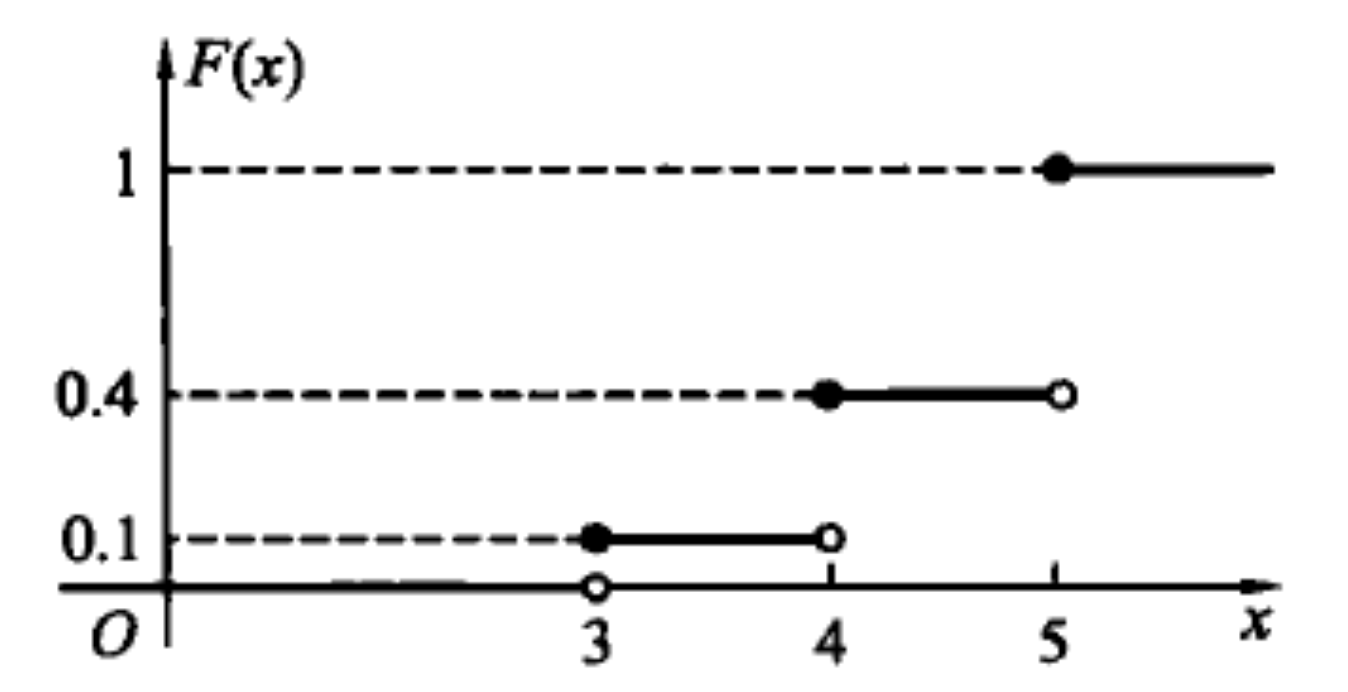
\includegraphics[width=0.5\textwidth]{pic1.png}
    \caption{F(x)}
\end{figure}

\section{2.1.7}
X的分布列为:

$$P(X=i)=\frac{C^i_{10}*C^{5-i}_{90}}{C_{100}^5},\quad i = 0,1,2,3,4,5.$$
当需要进行逐个检验时,意味着出现了至少一个不合格品,概率为:
$$P(X\geq 1)=1-P(X=0)=0.416$$
\section{2.1.9}
$$P(X<2)=F(2)=ln2=0.693$$
$$P(0<X\leq 3)=F(3)-F(0)=1$$
$$P(2<X\leq 2.5)=F(2.5)-F(2)=ln(2.5)-ln(2)=0.223$$
\section{2.1.11}
分布列为:
\begin{table}[H]
\centering
\begin{tabular}{c|ccc}
X & 2   & 3   & 4   \\
P & 0.3 & 0.4 & 0.3
\end{tabular}
\end{table}
分布函数为:
\begin{equation}
F(x)=P(X\leq x)=
\begin{cases}
0, &x<2,\\
0.3, &2\leq x < 3,\\
0.7, &3\leq x < 4,\\
1, &x\geq 4
\end{cases}
\end{equation}
$$P(X<2)=F(2)=0$$
$$P(X>4)=1-F(4)=0$$
\section{2.1.12}
密度函数在整个定义域上分为四段,因此分布函数也要分四段描述,根据定义对密度函数进行积分,得到分布函数为:
\begin{equation}
F(x)=
\begin{cases}
0, &x<-1,\\
\frac{x^2}{2}+x+0.5, &-1\leq x < 0,\\
-\frac{x^2}{2}+x+0.5, &0\leq x < 1,\\
1, &x\geq 1
\end{cases}
\end{equation}

\section{2.1.19}
因为p(x)为偶函数,所以有:
$$p(-x)=p(x)$$
$$\int^{+\infty}_{-\infty}p(x)dx=2\int^{+\infty}_{0}p(x)dx=1$$
(1)变量替换
$$F(-a)=\int^{-a}_{-\infty}p(x)dx=\int_{+\infty}^{a}p(t)d(-t)=\int^{+\infty}_{a}p(t)dt=1-F(a)$$
$$F(-a)=\int^{+\infty}_{a}p(t)dt=\int^{+\infty}_{0}p(t)dt-\int^{a}_{0}p(t)dt=0.5-\int^{a}_{0}p(x)dx$$

(2)
$$P(|X|<a)=P(-a<X<a)=F(a)-F(-a)=F(a)-[1-F(a)]=2F(a)-1$$

(3)
\begin{align*}
P(|X|>a)&=P(X<-a)+P(X>a)\\
&=F(-a)+1-F(a)\\
&=1-F(a)+1-F(a)\\
&=2[1-F(a)]
\end{align*}

\section{补充题}
父亲要孩子们去后院整理杂物,于是他的3个孩子就用每人同时抛一个硬币来决定谁去整理,他们规定,谁抛出的面与另外两人的不同就谁去整理,若三人抛出的面相同则需重抛,直到选出为止,假设硬币出现正面的概率为p,出反面为q,求:

1.他们抛了不到n轮就能选出人的概率;

2.若p=0.5,最少要抛多少轮,才能以0.95以上的概率可以选出人来。

解:

前提:p+q=1

设事件A为“三次抛硬币面相同”,则有:
$$P(A)=p^3+q^3$$

设事件$B_n$为“抛了n轮没有选出人”,则有:
$$P(B_n)=P(A)^{n},\quad n=1,2,3,...$$

因此他们抛了不到n轮就能选出人的概率为:
$$P=1-P(B_{n-1})=1-(p^3+q^3)^{n-1}, \quad n=2,3,4,...$$ 

因为$p=0.5=q$,因此$P(A)=0.25$,若以0.95以上的概率选出人来,需要$P(A)^n<1-0.95=0.05$。
当n=2时,$P(A)^n=0.0625$;当n=3时,$P(A)^n=0.015625$。
连续抛硬币3轮仍然没有选中人的概率为$(0.25)^3=0.015625$,因此最少抛3轮才能以0.95以上的概率选出人来。
\end{document}